\documentclass{article}
\usepackage[utf8x]{inputenc}
\usepackage{ucs}
\usepackage{amsmath} 
\usepackage{amsfonts}
\usepackage{upgreek}
\usepackage[english,russian]{babel}
\usepackage{graphicx}
\usepackage{float}
\usepackage{textcomp}
\usepackage{hyperref}
\usepackage{geometry}
  \geometry{left=2cm}
  \geometry{right=1.5cm}
  \geometry{top=1cm}
  \geometry{bottom=2cm}
\usepackage{tikz}
\usepackage{ccaption}
\usepackage{multicol}
%\setlength{\columnsep}{1.5cm}
%\setlength{\columnseprule}{0.2pt}
\usepackage{listings}

\begin{document}
\pagenumbering{gobble}

\lstset{
  language=C,                % choose the language of the code
  basicstyle=\linespread{1.1}\ttfamily,
  columns=fixed,
  fontadjust=true,
  basewidth=0.5em,
  keywordstyle=\color{blue}\bfseries,
  commentstyle=\color{gray},
  stringstyle=\ttfamily\color{orange!50!black},
  showstringspaces=false,
  %numbers=false,                   % where to put the line-numbers
  numbersep=5pt,
  numberstyle=\tiny\color{black},
  numberfirstline=true,
  stepnumber=1,                   % the step between two line-numbers.        
  numbersep=10pt,                  % how far the line-numbers are from the code
  backgroundcolor=\color{white},  % choose the background color. You must add \usepackage{color}
  showstringspaces=false,         % underline spaces within strings
  captionpos=b,                   % sets the caption-position to bottom
  breaklines=true,                % sets automatic line breaking
  breakatwhitespace=true,         % sets if automatic breaks should only happen at whitespace
  xleftmargin=.2in,
  extendedchars=\true,
  keepspaces = true,
}
\lstset{literate=%
   *{0}{{{\color{red!20!violet}0}}}1
    {1}{{{\color{red!20!violet}1}}}1
    {2}{{{\color{red!20!violet}2}}}1
    {3}{{{\color{red!20!violet}3}}}1
    {4}{{{\color{red!20!violet}4}}}1
    {5}{{{\color{red!20!violet}5}}}1
    {6}{{{\color{red!20!violet}6}}}1
    {7}{{{\color{red!20!violet}7}}}1
    {8}{{{\color{red!20!violet}8}}}1
    {9}{{{\color{red!20!violet}9}}}1
}


\title{Семинар \#12: Двумерный динамический массив. Связный список.\vspace{-5ex}}\date{}\maketitle

\section*{Часть 1: Изменение указателя внутри функции}

\subsection*{Передача обычных переменных из функций}
Чтобы лучше понять как передавать из функции указатель на данные, вспомним две возможности передачи из функции обычной переменной. Это можно сделать через возвращаемое значение или через аргумент-указатель.

\begin{multicols}{2}
\textbf{Способ 1:}\\
Просто возвращаем
\begin{lstlisting}
#include <stdio.h>
int f() {
    return 123;
}

int main() {
    int a = f();
    printf("%i\n", a);
}
\end{lstlisting}

\columnbreak

\textbf{Способ 2:}\\
Передаём указатель на нашу переменную.\\
Изменяем переменную, используя указатель
\begin{lstlisting}
#include <stdio.h>
void f(int* p) {
    *p = 123;
}
int main() {
    int a;
    f(&a);
    printf("%i\n", a);
}
\end{lstlisting}
\end{multicols}


\subsection*{Передача указателя на данные в Куче из функции}
Оба этих способа работают и для передачи из функции указателя. Только в этом случае тип возвращаемой переменной будет \texttt{int*}, а не \texttt{int}. Допустим, мы захотели написать функцию, которая создаёт в Куче массив из трёх элементов (\texttt{10, 20} и \texttt{30}) и передаёт указатель на этот массив.
\begin{multicols}{2}
\textbf{Способ 1:}
\begin{lstlisting}
#include <stdio.h>
#include <stdlib.h>

int* f() {
    int* p = malloc(sizeof(int) * 3);
    p[0] = 10;
    p[1] = 20;
    p[2] = 30;
    return p;
}
int main() {
    int* a = f();
    for (int i = 0; i < 3; ++i)
        printf("%i\n", a[i]);
    free(a);
}
\end{lstlisting}

\columnbreak

\textbf{Способ 2:}
\begin{lstlisting}
#include <stdio.h>
#include <stdlib.h>

void f(int** pp) {
    *pp = malloc(sizeof(int) * 3);
    (*pp)[0] = 10;
    (*pp)[1] = 20;
    (*pp)[2] = 30;
}
int main() {
    int* a;
    f(&a);
    for (int i = 0; i < 3; ++i)
        printf("%i\n", a[i]);
    free(a);
}
\end{lstlisting}
\end{multicols}

\subsection*{Задача:}
\begin{itemize}
\item Напишите 2 функции, которые будут выделять память и передавать указатель на массив в Куче, содержащий первые 10 квадратов натуральных чисел. Одна функция должна просто возвращать указатель, а вторая принимать адрес указателя и задавать его нужным значением.
\end{itemize}

\newpage
\section*{Часть 2: Двумерный динамический массив}
В стандартной библиотеке нет специальных средств по созданию двумерных массивов в Куче. Но есть 2 варианта для создания
такого массива с использованием динамического выделения одномерных массивов:
\begin{enumerate}
\item Вместо создания двумерного динамического массива размером \texttt{n} на \texttt{m} можно создать одномерный динамический массив размера \texttt{n * m} и работать с ним.
Это хороший вариант, когда длины всех строк массива равны или примерно равны и не меняются.
\item Создать динамический массив из указателей, каждый указатель будет 
соответствовать строке. Затем, для каждой строки динамически выделить столько памяти,
сколько нужно. При этом нам нужно будет создать отдельный динамический массив(\texttt{sizes}), который будет хранить
размеры каждой строки. Схема такого массива представлена на рисунке:
\end{enumerate}
\begin{center}
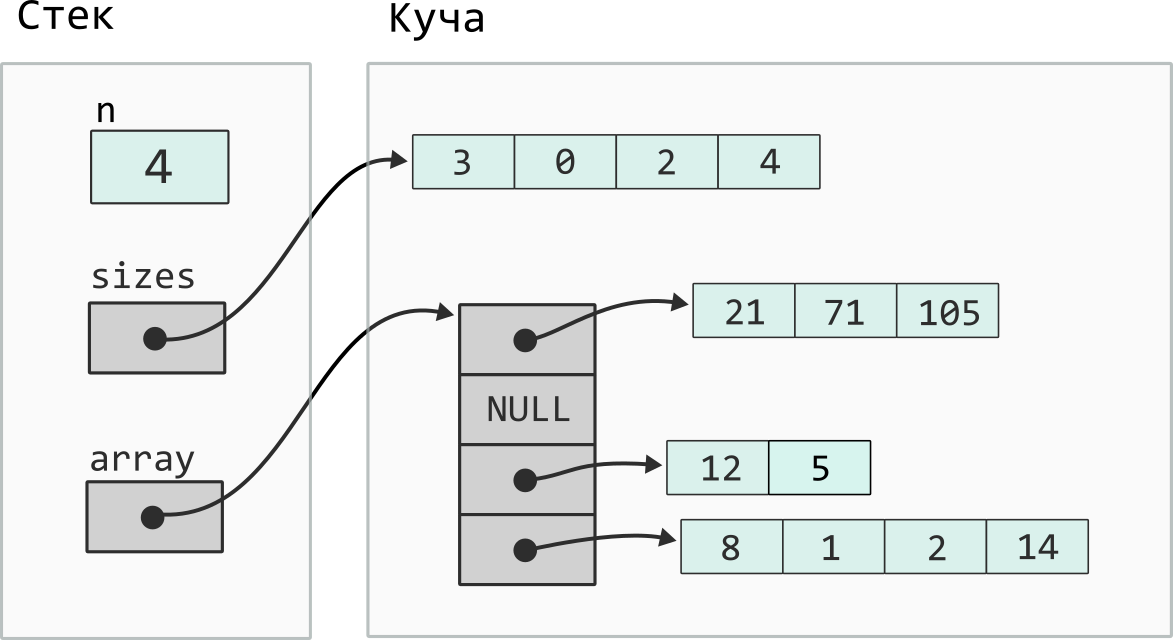
\includegraphics[scale=0.9]{../images/two_dim_dynamic_array.png}
\end{center}

\subsection*{Задачи}
\begin{itemize}


\item Напишите код, который будет выделять память в Куче и инициализировать её в соответствии со схемой на рисунке. Весь код должен быть в функции \texttt{main}.
\item Напишите функцию \texttt{void print\_two\_dim\_array(int n, int* sizes, int** array)} - печать.
\item Напишите функцию \texttt{void inc\_two\_dim\_array(int n, int* sizes, int** array)} - прибавить \texttt{1} ко всем элементам двумерного динамического массива.
\item Напишите \texttt{void delete\_two\_dim\_array(int n, int* sizes, int** array)} - освобождение памяти.
\item Напишите функцию \texttt{void create\_my\_two\_dim\_array(int* p\_n, int** p\_sizes, int*** p\_array)}, которая будет создавать в Куче двумерный динамический массив, инициализировать его в соответствии с рисунком и записывать значения \texttt{n}, \texttt{sizes} и \texttt{array} по передаваемым адресам \texttt{p\_n}, \texttt{p\_sizes} и \texttt{p\_array} соответственно. Вызовите эту функцию из функции \texttt{main}.
\item В файле \texttt{numbers.txt} содержится представление двумерного массива с разной длиной строк. В первой строке содержится число \texttt{n}, в следующей строке содержится массив \texttt{sizes} и в следующих \texttt{n} строках содежится сам массив. Напишите функцию\\
\texttt{void load\_two\_dim\_array(char filename[], int* p\_n, int** p\_sizes, int*** p\_array)}, \\
которая будет читать эти числа из файла под названием \texttt{filename} и записывать их в двуменый динамический массив. Эта функция сама должна выделять необходимую память.

\end{itemize}
\newpage
\section*{Часть 3: Связный список}
Создадим структуру \texttt{Node}, которая будет содержать:
\begin{itemize}
\item \textbf{Данные}: одно или несколько полей каких-угодно типов. В данном случае это 1 переменная \texttt{value}.
\item \textbf{Связь}: указатель \texttt{next} на структуру того же типа \texttt{Node}.
\end{itemize}
\begin{center}
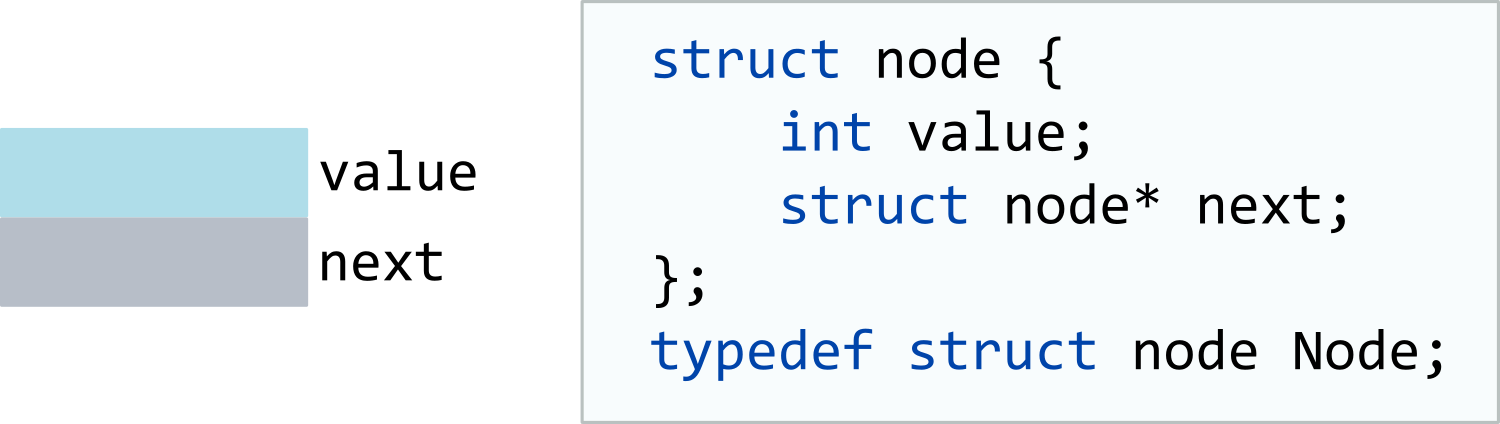
\includegraphics[scale=0.8]{../images/structlist.png}
\end{center}

Используя такую структуру, можно создать Связный список:
\begin{center}
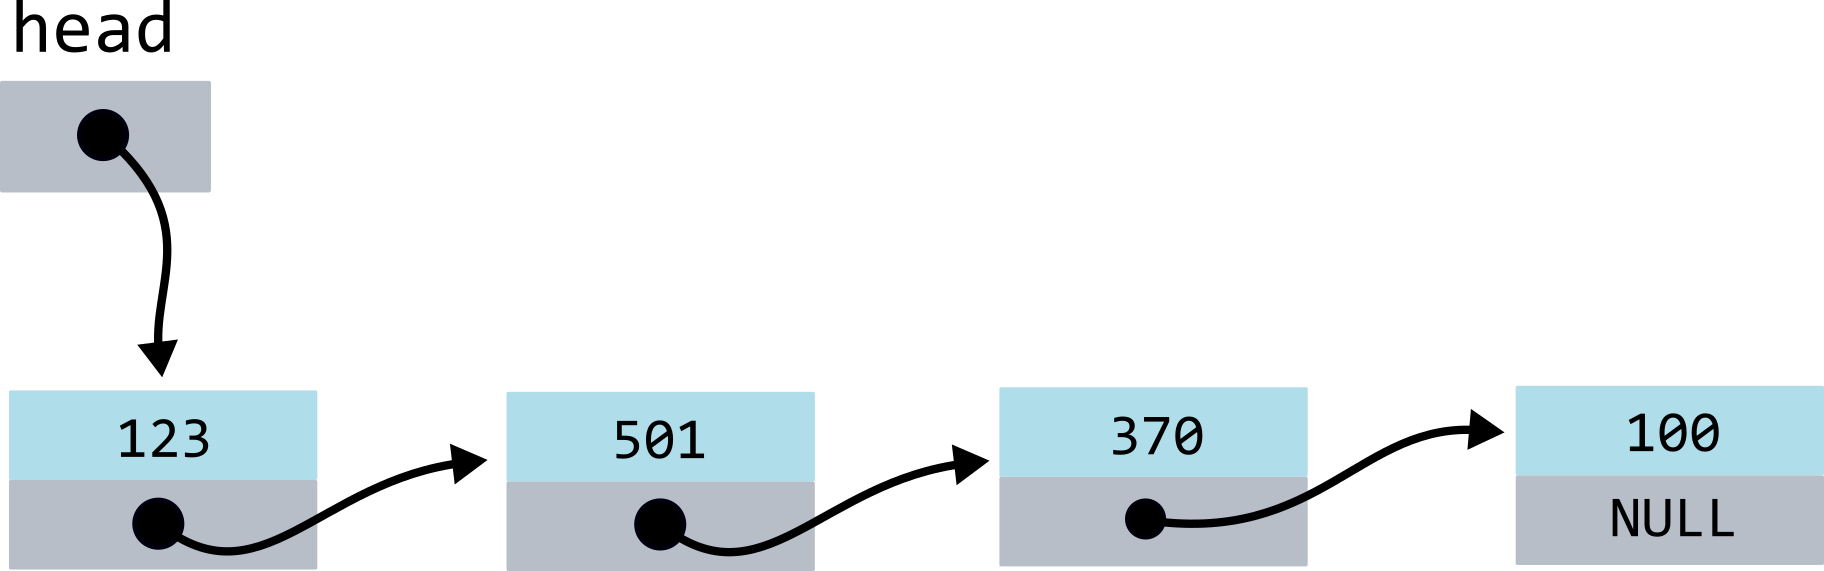
\includegraphics[scale=0.8]{../images/codelist/codelist_only.png}
\end{center}
\textit{Примечание}: \texttt{NULL} - это просто константа равная 0. Её используют вместо нуля для указателей, чтобы различать числовые переменные и указатели.\\

В нашем случае указатель \texttt{head} будет зраниться в сегменте Стек, а все элементы будут выделяться динамически и, соответственно, храниться в сегменте Куча. Пустой связный список будет представлять собой просто один указатель \texttt{head}, равный \texttt{NULL}.

\subsection*{Вычислительные сложности операций со списком:}
\begin{center}
\begin{tabular}{ c c c }
 Операция & Массив & Односвязный список \\ 
 \hline
 Доступ по номеру & $O(1)$ & $O(N)$  \\
 Поиск & $O(N)$ & $O(N)$  \\    
 Вставка в начало & $O(N)$ & $O(1)$  \\
 Вставка в конец & $O(1)$ & $O(N)$  \\
 \begin{tabular}{@{}c@{}}Вставка в конец если известен \\ указатель на последний элемент\end{tabular} & $O(1)$ & $O(1)$  \\
 Вставка в середину & $O(N)$ & $O(N)$  \\
 \begin{tabular}{@{}c@{}}Вставка в середину если известен \\ указатель на предыдущий элемент\end{tabular} & $O(N)$ & $O(1)$  \\  
\end{tabular}
\end{center}

Чему равны вычислительные сложности следующих операций:
\begin{itemize}
\item Нахождение размера списка. Что можно сделать, чтобы нахождение размера выполнялось быстрее?
\item Удаление элемента из начала списка.
\item Удаление элемента из конца списка. Что нужно знать, чтобы эта операция выполнялась быстрее?
\item Удаление элемента из середины списка. Что нужно знать, чтобы эта операция выполнялась быстрее?
\end{itemize}

\newpage
\subsection*{Задание}
Начальный код в файле \texttt{list.c}. Там уже написано 3 функции:
\begin{itemize}
\item \texttt{Node* list\_create()} -- инициализирует список (создаёт и возвращает список нулевого размера). Эта функция просто возвращает \texttt{NULL}. Зачем нужна такая простая функция? Она нужна для согласованности с реализациями других структур данных. Например, при реализации хеш-таблицы у нас будет более сложная функция \texttt{hashtable\_create}, которая будет создавать хеш-таблицу.
\item \texttt{void list\_add\_last(Node** p\_head, int x)} -- добавляет элемент x в конец списка. Также эта функция подробно разобрана в презентации.
\item \texttt{void list\_print(const Node* head, char separator[])} -- распечатывает все элементы списка, разделённые строкой \texttt{separator}. 
\end{itemize}

Можно заметить, что в одни функции передаётся сам указатель \texttt{head}, а в другие указатель на \texttt{head}, который называется \texttt{p\_head}. Это связано с тем, что некоторые функции должны менять само значение \texttt{head} и, чтобы это сделать, нужно передать в функцию указатель на \texttt{head}. Например, если список пуст и \texttt{head == NULL}, то после вызова функции  \texttt{list\_add\_last} указатель \texttt{head} должен измениться и указывать на новый элемент. Схематическое изображение выделенной памяти в случае передачи в функцию указателя на \texttt{head}:


\begin{center}
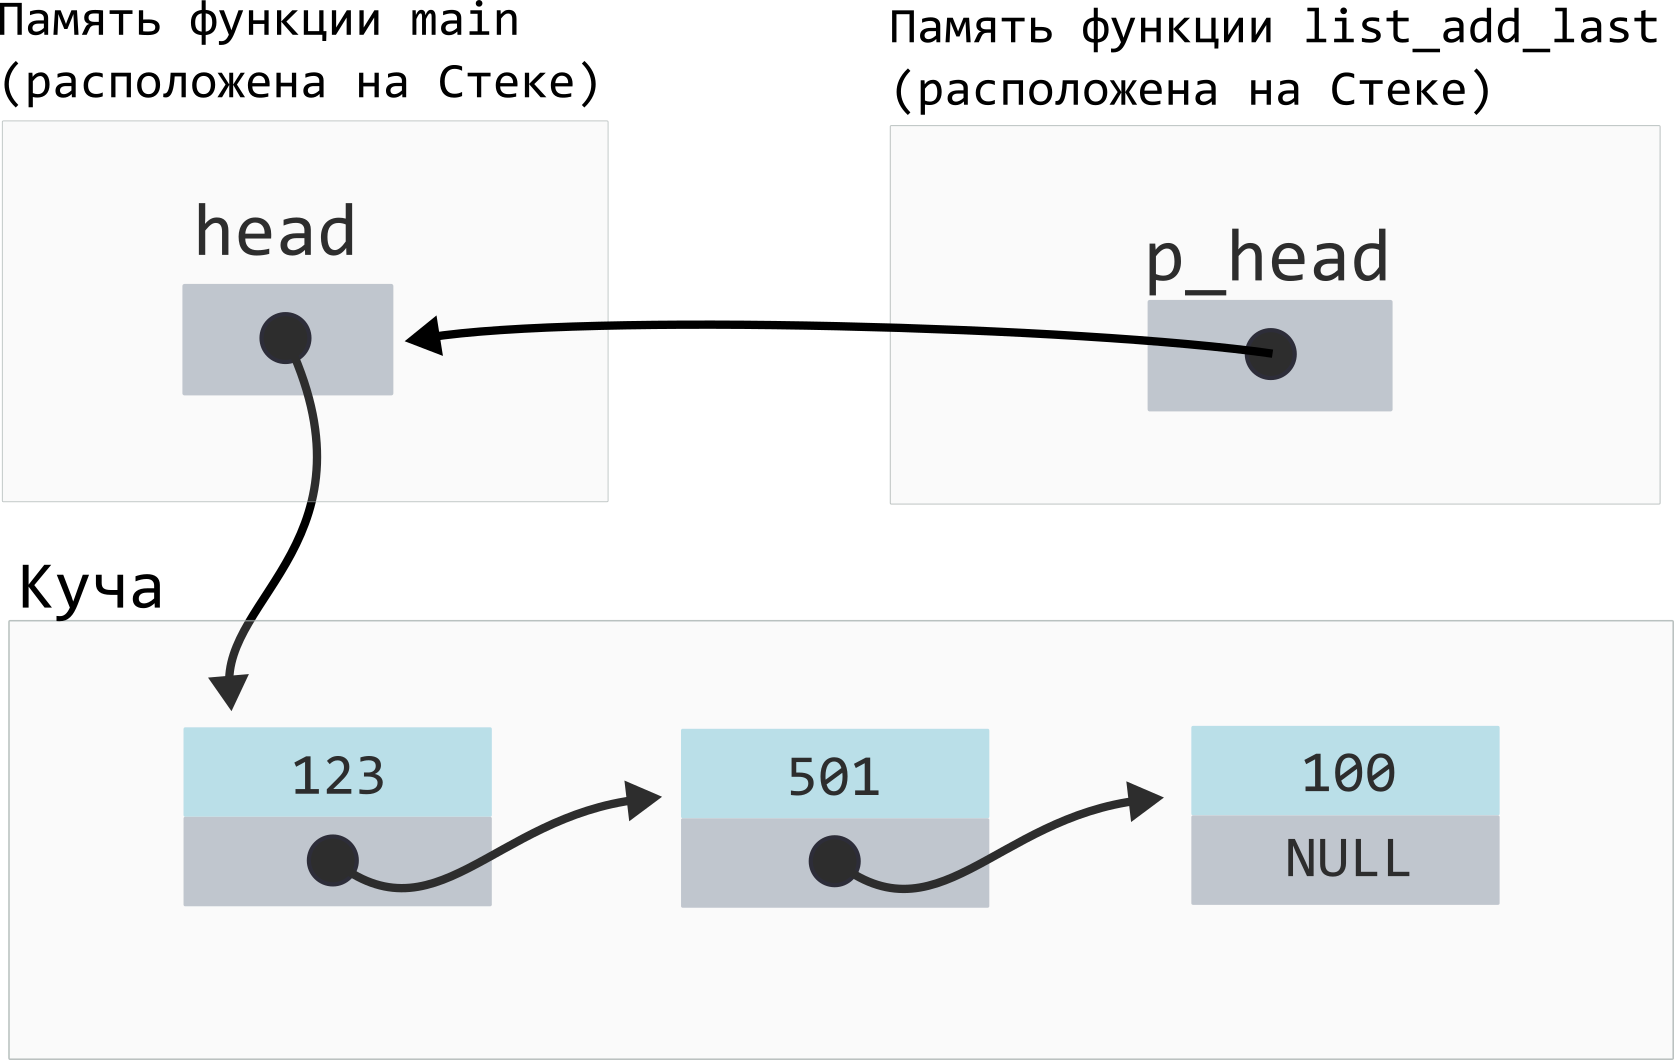
\includegraphics[scale=0.8]{../images/p_head.png}
\end{center}

\subsection*{Напишите следующие функции для работы со связным списком:}
\begin{itemize}
\item \texttt{void list\_add\_first(Node** p\_head, int x)} -- добавляет элемент x в начало списка. Чтобы добавить элемент, нужно для начала выделить необходимое количество памяти под этот элемент, затем задать поля нового элемента таким образом, чтобы он указывал на начало списка. В конце нужно поменять значение указателя \texttt{head}, используя \texttt{p\_head}.
\item \texttt{int list\_remove\_first(Node** p\_head)} -- удаляет элемент из начала списка и возвращает его значение. Не забудьте изменить \texttt{*p\_head}.

\item \texttt{int list\_remove\_last(Node** p\_head)} -- удаляет элемент из конца списка и возвращает его значение. 
\item \texttt{size\_t list\_size(const Node* head)} -- возвращает количество элементов списка.
\item \texttt{void list\_destroy(Node* head)} -- освобождает всю память, выделенную под список. Так как память выделялась под каждый элемент отдельно, то освобождать нужно также каждый элемент по отдельности.

\item \texttt{void list\_reverse(Node** p\_head)} -- переворачивает связный список. Первый элемент становится последним, а последний первым. В данной задаче вам не нужно перемещать элементы \texttt{value} или сами структуры. Нужно просто изменить указатели. Эта задача разобрана в презентации.

\item \texttt{void list\_concatenate(Node** p\_head1, const Node* head2)}, которая добавляет второй связный список в конец первого. Особенно рассмотрите случай когда первый список -- пуст.


\item Добавить \texttt{typedef}-синоним для элементов связного списка. (функция для печати списка при этом может стать недейсвительной, так как там используется спецификатор \texttt{\%i}).
\item Вынести всю реализацию связного списка в отдельный файл \texttt{list.h}. Подключить этот файл к вашему \texttt{.c} файлу.
\item Реализовать абстрактный тип данных стек(Stack) на основе связного списка. Реализация должна находится в файле \texttt{stack.h}.
\end{itemize}

\subsection*{Цикл в связном списке:}
Если, вдруг, последний элемент связного списка имеет поле \texttt{next}, которое не равно нулю, а содержит указатель на один из элементов списка, то в списке образуется цикл. На изображении показано как это выглядит. 
\begin{center}
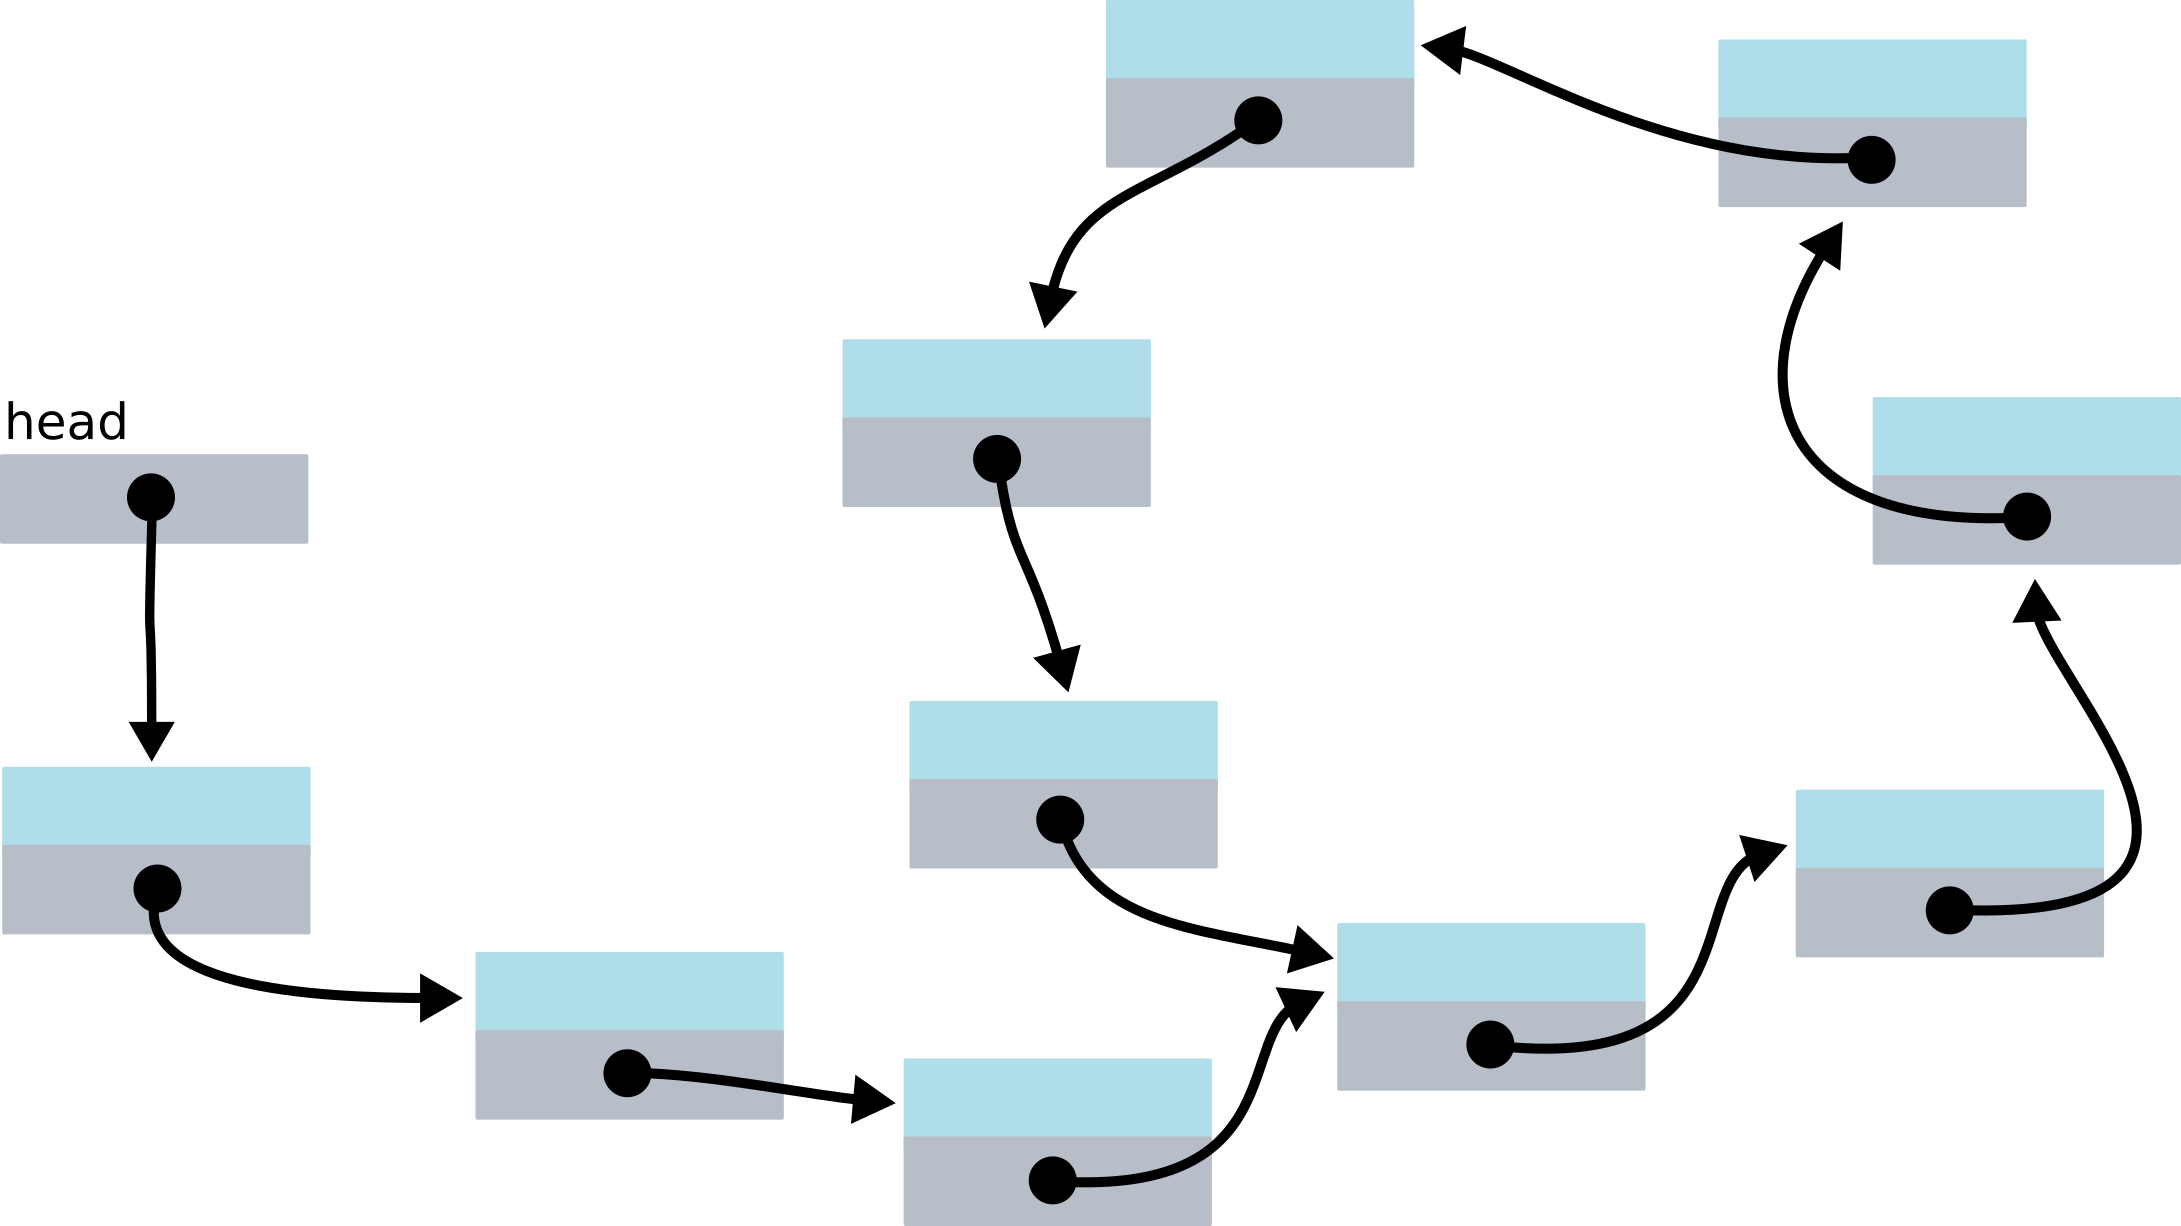
\includegraphics[scale=0.77]{../images/list_loop_2.png}
\end{center}

\begin{itemize}
\item Написать функцию \texttt{Node* create\_my\_looped\_list()}, которая будет создавать в куче связный список, состоящий из трёх элементов (\texttt{10}, \texttt{20} и \texttt{30}). При этом указатель \texttt{next} последнего элемента должен указывать на первый элемент. Что будет если передать такой связный список в функцию \texttt{list\_print}.
\item Написать функцию \texttt{int list\_is\_loop(Node* head)}, которая проверяет, если в связном списке цикл. Функция должна вернуть \texttt{1} если в списке есть цикл и \texttt{0}, если его нет.
\item Написать функцию \texttt{void list\_fix\_loop(Node* head)}, которая проверяет, если в связном списке цикл. И если цикл есть, то она размыкает его. То есть устанавливает поле \texttt{next} последнего элемента значением \texttt{NULL}.
\end{itemize}\end{document}